\subsection{Introducción}

  \paragraph{}El usuario \textit{Asesor} se encarga de gestionar tanto su
  información persona como la de cierta información sobre los alumnos a los que
  presta o ha prestado asesoría. La información que puede gestionar este usuario
  se menciona a continuación:

  \begin{itemize}
   \item Alumnos (asesorados)
   \item Plantillas
   \begin{itemize}
      \item Plantillas oficiales
      \item Preguntas oficiales
      \item Plantillas de asesor
      \item Preguntas de asesor
   \end{itemize}
   \item Reuniones
   \begin{itemize}
      \item Reuniones individuales
      \item Reuniones grupales
   \end{itemize}
  \end{itemize}

  \paragraph{}Además, a este usuario le estará permitido modificar cierta
  información personal; por ejemplo, su contraseña o correo electrónico.

  \paragraph{}Para acceder a cada uno de estos elementos, se podrá realizar de
  dos formas distintas:

  \begin{itemize}
   \item Mediante el menú principal. Este menú es el que refleja la figura
   \ref{capturaMenuPrincipalAsesor}.

  \begin{figure}[!ht]
    \begin{center}
      
\includegraphics[scale=0.55]{4.Funcionamiento_Aplicacion/4.3.Gestion/4.3.3.Asesor/4.3.3.1.Introduccion/menu_principal.png}
      \caption{Captura del menú principal del usuario \textit{Asesor}.}
      \label{capturaMenuPrincipalAsesor}
    \end{center}
  \end{figure}

   \item Mediante el menú lateral. Este menú es el que refleja la figura
   \ref{capturaMenuLateralAsesor}.

   \begin{figure}[!ht]
    \begin{center}
      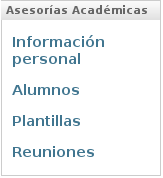
\includegraphics[scale=0.55]{4.Funcionamiento_Aplicacion/4.3.Gestion/4.3.3.Asesor/4.3.3.1.Introduccion/menu_lateral.png}
      \caption{Captura del menú lateral del usuario \textit{Asesor}.}
      \label{capturaMenuLateralAsesor}
    \end{center}
  \end{figure}

  \end{itemize}

  \paragraph{}A continuación, se pasa a detallar todos y cada uno de los
  elementos que este usuario puede gestionar en el sistema.
